% https://tex.stackexchange.com/a/52766/173708
\documentclass{standalone}

\usepackage{tikz}
\usetikzlibrary{shapes,positioning,arrows,calc}

\begin{document}

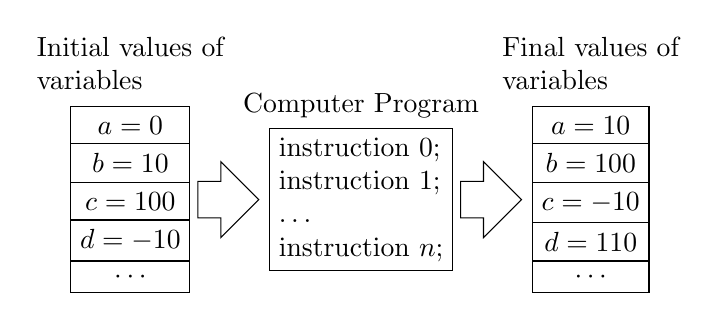
\begin{tikzpicture}[stack/.style={
  rectangle split, rectangle split parts=5, draw, anchor=center},
  myarrow/.style={single arrow, draw=none}]

  \node [stack] (ini)  {$a=0$\nodepart{two}$b=10$%
    \nodepart{three}$c=100$\nodepart{four}$d=-10$\nodepart{five}$\cdots$};

  \node [draw,rectangle,align=left,right=of ini,label=above:{Computer Program}] (mid)
    {instruction 0;\\ instruction 1;\\$\ldots$\\instruction $n$;};

  \node [stack,right=of mid] (fin) {$a=10$\nodepart{two}$b=100$%
    \nodepart{three}$c=-10$\nodepart{four}$d=110$\nodepart{five}$\cdots$};

  \node [above=of ini,anchor=north,align=left] {Initial values of\\variables};
  \node [above=of fin,anchor=north,align=left] {Final values of\\variables};

  \node [myarrow,draw,anchor=west] at ($(ini.east)+(2.5pt,0)$) {\phantom{te}} ;
  \node [myarrow,draw,anchor=west] at ($(mid.east)+(2.5pt,0)$) {\phantom{te}} ;

\end{tikzpicture}

\end{document}